\documentclass{article}[12 pt]
\author{Berkay VURKAN}
%Increase the text height
\newcommand\tab[1][0.5cm]{\hspace*{#1}}
\usepackage{textcomp}
\usepackage{amssymb}
\usepackage{amsmath}
\usepackage{multirow}
\usepackage[margin=0.5in]{geometry}
\usepackage[utf8]{inputenc}
\usepackage{makecell}

\usepackage{pgfplots}
\pgfplotsset{width=10cm,compat=1.9}
%\usepgfplotslibrary{external}
%\tikzexternalize

\begin{document}
	\paragraph{\large{Networkx library vs. DiGraph class}}
	\begin{center}
		\begin{tabular}{ |c|c|c|l| }
			\hline
			\multicolumn{4}{ |c| }{\large{\textsc{Stats}}} \\
			\hline
			\textbf{\# of vertices} &\textbf{type} & \textbf{sample paths} & \textbf{Elapsed Time} \\ \hline
			\multirow{10}{*}{500} & Networkx & ['dubbers', 'neuters', 'peptone'] & $4.8\times 10^{-5}$ s\\
			& DiGraph & [('dubbers', 'boreens'), ('boreens', 'peptone')] & $2.5\times 10^{-2}$ s\\
			& Networkx & ['caddice', 'angelic', 'cyanate'] & $3.7\times 10^{-5}$ s\\
			& DiGraph & [('caddice', 'astelic'), ('astelic', 'cyanate')] & $8.3\times 10^{-3}$ s\\
			& Networkx & ['hokonui', 'ruction'] & $2.5\times 10^{-5}$ s\\
			& DiGraph & [('hokonui', 'ruction')] & $1.3\times 10^{-3}$ s\\
			& Networkx & ['sideral', 'salutes', 'hocuses'] & $6.5\times 10^{-5}$ s\\
			& DiGraph & [('sideral', 'becurls'), ('becurls', 'hocuses')] & $4.5\times 10^{-2}$ s\\
			& Networkx & ['sheepos', 'powters', 'madwort'] & $4.7\times 10^{-5}$ s\\
			& DiGraph & [('sheepos', 'drowses'), ('drowses', 'madwort')] & $6.1\times 10^{-2}$ s\\  \hline
			
			\multirow{10}{*}{1000} & Networkx & ['gorgons', 'informs'] & $4.7\times 10^{-5}$ s\\
			& DiGraph & [('gorgons', 'informs')] & $4.4\times 10^{-3}$ s\\
			& Networkx & ['maelids', 'stamper', 'erasure'] & $1.1\times 10^{-4}$ s\\
			& DiGraph & [('maelids', 'dustier'), ('dustier', 'erasure')] & $2.1\times 10^{-2}$ s\\
			& Networkx & ['planked', 'damsels', 'muskegs', 'gummous'] & $1.1\times 10^{-4}$ s\\
			& DiGraph & [('planked', 'plucker'), ('plucker', 'scourge'), ('scourge', 'gummous')] & $1.2$ s\\
			& Networkx &['althaea', 'petaras', 'jazzers'] & $5.5\times 10^{-5}$ s\\
			& DiGraph & [('althaea', 'stapler'), ('stapler', 'jazzers')] & $4.2\times 10^{-2}$ s\\
			& Networkx & ['patness', 'paeonic', 'flacons'] & $8.4\times 10^{-5}$ s\\
			& DiGraph & [('patness', 'parcels'), ('parcels', 'flacons')] & $1.5\times 10^{-2}$ s\\\hline
			
			\multirow{10}{*}{1500} & Networkx & ['folkmot', 'smooths', 'chromas'] & $1.2\times 10^{-4}$ s\\
			& DiGraph &[('folkmot', 'smooths'), ('smooths', 'chromas')] & $1.1\times 10^{-1}$ s\\
			& Networkx & ['plating', 'lotions', 'outtold'] & $9.3\times 10^{-5}$ s\\
			& DiGraph & [('plating', 'lotions'), ('lotions', 'outtold')] & $8.1\times 10^{-1}$ s\\
			& Networkx & ['remodel', 'clotter', 'outtold'] & $9.2\times 10^{-5}$ s\\
			& DiGraph & [('remodel', 'outedge'), ('outedge', 'outtold')] & $2.7\times 10^{-1}$ s\\
			& Networkx &['legongs', 'consult', 'mutines'] & $9.1\times 10^{-5}$ s\\
			& DiGraph & [('legongs', 'skeeing'), ('skeeing', 'mutines')] & $4.9\times 10^{-2}$ s\\
			& Networkx & ['nursery', 'downers', 'redcaps'] & $8.8\times 10^{-5}$ s\\
			& DiGraph & [('nursery', 'remoras'), ('remoras', 'redcaps')] & $1.1\times 10^{-1}$ s\\\hline
			
			\multirow{10}{*}{2000} & Networkx & ['relaxin', 'rancing', 'bonings'] & $2.4\times 10^{-4}$ s\\
			& DiGraph &[('relaxin', 'ironise'), ('ironise', 'bonings')] & $4.7\times 10^{-1}$ s\\
			& Networkx &['abridge', 'hastier', 'futures'] & $1.7\times 10^{-4}$ s\\
			& DiGraph & [('abridge', 'hastier'), ('hastier', 'futures')] & $1.1$ s\\
			& Networkx & ['airings', 'interim', 'cometic'] & $1.3\times 10^{-4}$ s\\
			& DiGraph & [('airings', 'caniest'), ('caniest', 'cometic')] & $1.5$ s\\
			& Networkx &['blawort', 'maltier', 'pilcher'] & $8.2\times 10^{-5}$ s\\
			& DiGraph & [('blawort', 'railbed'), ('railbed', 'pilcher')] & $5.8\times 10^{-1}$ s\\
			& Networkx & ['chibols', 'miscode', 'rewinds'] & $9.4\times 10^{-5}$ s\\
			& DiGraph & [('chibols', 'shilled'), ('shilled', 'rewinds')] & $5.8\times 10^{-2}$ s\\\hline
			
			\multirow{10}{*}{2500} & Networkx & ['midmost', 'posties', 'lysines'] & $9.4\times 10^{-5}$ s\\
			& DiGraph & [('midmost', 'emetins'), ('emetins', 'lysines')] & $9.0\times 10^{-2}$ s\\
			& Networkx & ['zingaro', 'santero', 'swathed'] & $1.2\times 10^{-4}$ s\\
			& DiGraph & [('zingaro', 'easting'), ('easting', 'swathed')] & $2.7$ s\\
			& Networkx & ['pigtail', 'stabile', 'burbles'] & $1.5\times 10^{-4}$ s\\
			& DiGraph & [('pigtail', 'lairise'), ('lairise', 'burbles')] & $3.1$ s\\
			& Networkx & ['nutwood', 'buncoed', 'pinched'] & $1.2\times 10^{-4}$ s\\
			& DiGraph & [('nutwood', 'pouncet'), ('pouncet', 'pinched')] & $1.5$ s\\
			& Networkx & ['andvile', 'ikebana', 'bagnios'] & $2.1\times 10^{-4}$ s\\
			& DiGraph & [('andvile', 'yodling'), ('yodling', 'bagnios')] & $8.9\times 10^{-1}$ s\\
			\hline
		\end{tabular}
	\end{center}
	\begin{center}
		\begin{tabular}{ |c|c|c|l| }
			\hline
			\multicolumn{4}{ |c| }{\large{\textsc{Stats}}} \\
			\hline
			\textbf{\# of vertices} &\textbf{type} & \textbf{sample paths} & \textbf{Elapsed Time} \\ \hline
			\multirow{10}{*}{3000} & Networkx & ['lensmen', 'gyrenes', 'garnish'] & $2.0\times 10^{-4}$ s\\
			& DiGraph & [('lensmen', 'manwise'), ('manwise', 'garnish')] & $1.2$ s\\
			& Networkx & ['bogyman', 'decagon', 'scooped', 'pickers'] & $5.1\times 10^{-4}$ s\\
			& DiGraph & [('bogyman', 'bausond'), ('bausond', 'debarks'), ('debarks', 'pickers')] & $28.4$ s\\
			& Networkx & ['gollans', 'litoral', 'mooktar'] & $3.2\times 10^{-4}$ s\\
			& DiGraph & [('gollans', 'megaron'), ('megaron', 'mooktar')] &$6.3\times 10^{-1}$ s\\
			& Networkx & ['lording', 'poitrel'] & $9.2\times 10^{-5}$ s\\
			& DiGraph & [('lording', 'poitrel')] & $6.2\times 10^{-3}$ s\\
			& Networkx & ['realtor', 'carpale'] & $6.1\times 10^{-4}$ s\\
			& DiGraph & [('realtor', 'carpale')] & $7.3\times 10^{-2}$ s\\  \hline
			
			\multirow{10}{*}{3500} & Networkx & ['broaden', 'pirogen'] & $2.2\times 10^{-4}$ s\\
			& DiGraph & [('broaden', 'pirogen')] & $3.9\times 10^{-2}$ s\\
			& Networkx & ['cagmags', 'impacts', 'poetise']  & $2.1\times 10^{-4}$ s\\
			& DiGraph & [('cagmags', 'atomics'), ('atomics', 'poetise')] & $3.3$ s\\
			& Networkx & ['aneared', 'reamers', 'bewared'] & $2.7\times 10^{-4}$ s\\
			& DiGraph & [('aneared', 'radioed'), ('radioed', 'bewared')] & $2.7\times 10^{-1}$ s\\
			& Networkx & ['hilloed', 'birthed', 'bartsia'] & $1.9\times 10^{-4}$ s\\
			& DiGraph & [('hilloed', 'lathier'), ('lathier', 'bartsia')] & $8.4$ s\\
			& Networkx & ['jihadis', 'haziest', 'heezing'] & $1.0\times 10^{-4}$ s\\
			& DiGraph & [('jihadis', 'hayings'), ('hayings', 'heezing')] & $3.9\times 10^{-1}$ s\\\hline
			
			\multirow{10}{*}{4000} & Networkx & ['balista', 'kasbahs', 'splakes'] & $3.2\times 10^{-4}$ s\\
			& DiGraph & [('balista', 'pilaffs'), ('pilaffs', 'splakes')] & $6.3$ s\\
			& Networkx & ['goodmen', 'dogears', 'nocakes']  & $2.5\times 10^{-4}$ s\\
			& DiGraph & [('goodmen', 'songman'), ('songman', 'nocakes')] & $1.8$ s\\
			& Networkx & ['clacked', 'crestal', 'rebites'] & $1.7\times 10^{-4}$ s\\
			& DiGraph & [('clacked', 'batiked'), ('batiked', 'rebites')] & $6.1$ s\\
			& Networkx & ['blatest', 'wrestle', 'sleechy'] & $2.9\times 10^{-4}$ s\\
			& DiGraph & [('blatest', 'scantly'), ('scantly', 'sleechy')] & $1.2$ s\\
			& Networkx & ['dandler', 'garners'] & $6.0\times 10^{-5}$ s\\
			& DiGraph & [('dandler', 'garners')] & $1.5\times 10^{-1}$ s\\\hline
			
			\multirow{10}{*}{4500} & Networkx & ['surname', 'malmsey', 'stagily'] & $5.0\times 10^{-4}$ s\\
			& DiGraph & [('surname', 'irisate'), ('irisate', 'stagily')] & $2.8$ s\\
			& Networkx & ['laiding', 'lungans', 'nunatak']  & $4.9\times 10^{-4}$ s\\
			& DiGraph & [('laiding', 'latinas'), ('latinas', 'nunatak')] & $12.2$ s\\
			& Networkx & ['coverer', 'recoats', 'stopped'] & $2.4\times 10^{-4}$ s\\
			& DiGraph & [('coverer', 'revolts'), ('revolts', 'stopped')] & $1.5$ s\\
			& Networkx & ['cloning', 'eosinic', 'corvets']  & $2.4\times 10^{-4}$ s\\
			& DiGraph & [('cloning', 'logiest'), ('logiest', 'corvets')] & $3.0$ s\\
			& Networkx & ['degamis', 'disform', 'deposer'] & $3.9\times 10^{-4}$ s\\
			& DiGraph & [('degamis', 'defaste'), ('defaste', 'deposer')] & $4.0\times 10^{-1}$ s\\\hline
			
			\multirow{10}{*}{5000} & Networkx & ['chamiso', 'mashuas', 'asphalt'] & $2.7\times 10^{-4}$ s\\
			& DiGraph & [('chamiso', 'kamilas'), ('kamilas', 'asphalt')] & $1.1$ s\\
			& Networkx & ['injurer', 'pardine', 'ikebana'] & $2.2\times 10^{-4}$ s\\
			& DiGraph & [('injurer', 'nickers'), ('nickers', 'ikebana')] & $1.1$ s\\
			& Networkx & ['bardism', 'caritas'] & $4.6\times 10^{-5}$ s\\
			& DiGraph & [('bardism', 'caritas')] & $1.6\times 10^{-1}$ s\\
			& Networkx & ['affrets', 'easting', 'gnawing'] & $5.8\times 10^{-4}$ s\\
			& DiGraph & [('affrets', 'gannets'), ('gannets', 'gnawing')] & $50.4$ s\\
			& Networkx & ['gyrator', 'amorets', 'humites'] & $2.9\times 10^{-4}$ s\\
			& DiGraph & [('gyrator', 'amorets'), ('amorets', 'humites')] & $1.3$ s\\
			\hline
		\end{tabular}
	\end{center}
	\begin{center}
		\begin{tabular}{|l|c|c|}\hline
			\multicolumn{3}{ |c| }{\textsc{Means of Elapsed Times}} \\ \hline
			\diaghead{\theadfont Diag ColumnmnHead II}%
			{\textbf{Number}\\\textbf{of Vertices}}{\textbf{Types}}&
			\thead{\textbf{Networkx}}&\thead{\textbf{DiGraph}}\\ \hline
			500 & $4.5\times 10^{-5}$ s & $2.8\times 10^{-2}$ s \\    \hline
			1000 & $8.0\times 10^{-5}$ s & $2.5\times 10^{-1}$ s \\    \hline
			1500 & $9.3\times 10^{-5}$ s & $2.6\times 10^{-1}$ s \\    \hline
			2000 & $1.4\times 10^{-4}$ s & $7.5\times 10^{-1}$ s \\    \hline
			2500 & $1.5\times 10^{-4}$ s & $1.6$ s \\    \hline
			3000 & $2.4\times 10^{-4}$ s & $6.1$ s \\    \hline
			3500 & $2.5\times 10^{-4}$ s & $2.5$ s \\    \hline
			4000 & $2.2\times 10^{-4}$ s & $3.1$ s \\    \hline
			4500 & $3.7\times 10^{-4}$ s & $4.1$ s \\    \hline
			5000 & $2.8\times 10^{-4}$ s & $10.8$ s \\    \hline
		\end{tabular}
	\end{center}
	\begin{center}
			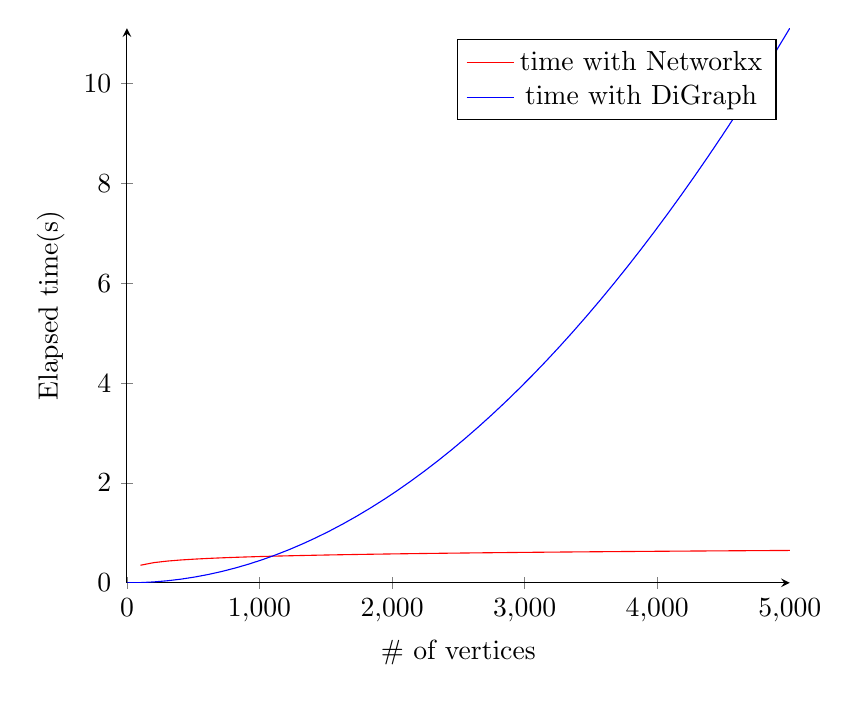
\begin{tikzpicture}
			\begin{axis}[
			axis lines = left,
			xlabel = {\# of vertices},
			ylabel = Elapsed time(s),
			]
			%Below the red parabola is defined
			\addplot [
			domain=0:5000, 
			samples=50, 
			color=red,
			]
			{ln(x)/ln(5*10^5)};
			\addlegendentry{time with Networkx}
			%Here the blue parabola is defined
			\addplot [
			domain=0:5000, 
			samples=50, 
			color=blue,
			]
			{(x/1500)^2};
			\addlegendentry{time with DiGraph}
			
			\end{axis}
			\end{tikzpicture}
	\end{center}
	\tab Datalara göre en anlamlı grafik yukarıdaki gibi oluşuyor.Vertex sayısının belirli bi  yerden sonraki artışı Networkx'i çok etkilemezken DiGraph bu durumdan oldukça etkileniyor.Görüldüğü üzere Networkx $ \varTheta lgN $ ile oldukça iyi çalışıyor :)
	
	
\end{document}